\chapter{绪论}
\section{引言}
文字和语音都是自然语言处理领域的研究对象。无论是比较早期的句法、词法分析,音素研究,还是诞生稍晚的针对语音内容的识别、拼接合成,对于文字和语音内容的研究可称得上互为表里。语音是文字可感知的信号载体,文字是语音内容的本质表示。
机器翻译一直以来都是自然语言处理领域针对不同语言文字的一项重要技术。对于机器翻译的研究最早始于20世纪30年代,它的发展一直与计算机技术、语言学和信息论等学科密切相关。从早期的字典匹配、结合专家知识的规则翻译等朴素方法,到结合概率统计学和语言学的统计机器翻译,再到近年来随着运算硬件性能提高和深度神经网络发展而兴起的神经机器翻译,机器翻译技术取得了世人瞩目的成功,这项技术本身也逐渐从学界中的理论发展走向工业界的落地实践。

自动歌曲翻译是神经机器翻译在这一基础上针对非常规语体的拓展性研究,这一任务旨在。

歌声合成则是由语音合成任务衍生而来。语音合成是仅以文本为输入、以梅尔特征图或声波波形为输出的生成任务,歌声合成和语音合成任务不同的是,其文本发声时所对应的音高和时长都为设定好的乐谱所限制。
歌声合成使得歌曲翻译结果的直观评测成为可能。同时,由于歌声合成可以承接歌曲翻译的输出结果而连接成为完整的、级联式的歌曲到歌声的翻译系统,这为歌曲翻译的实际应用打下了坚实的基础。
\section{国内外研究现状}
\subsection{自动歌曲翻译国内外研究现状}
\subsection{歌声合成国内外研究现状}
最初的歌声合成工作始于连接音频片段式~\citep{macon1997concatenation,kenmochi2007vocaloid}或基于隐马尔可夫统计模型的参数化~\citep{saino2006hmm,oura2010recent}方法。这些方法由于早期的硬件运算能力、算法研究等局限性,和现在的方法相比过程非常繁琐,而且合成的结果缺乏人声的灵动感和和谐感。近年来,深度学习蓬勃发展,在过去的几年中,基于深度神经网络的歌声合成系统逐渐成为研究主流。
%\citet{nishimura2016singing,blaauw2017neural,kim2018korean,nakamura2019singing,gu2020bytesing}
利用神经网络将上下文特征映射到声学特征。\citet{ren2020deepsinger}使用从音乐网站挖掘的演唱数据,成功构建具有实际落地潜力的歌声合成系统。\citet{blaauw2020sequence} 提出了一种基于Transformer的非自回归序列生成模型,相比自回归模型,可以更快速地进行模型推理,而且能避免自回归模型引起的暴露偏差问题。 Besides,
with the help of adversarial training, \citet{lee2019adversarially}~propose an end-to-end framework which directly generates linear-spectrograms. \citet{wu2020adversarially}~present a multi-singer SVS system with limited available recordings and improve the voice quality by adding multiple random window discriminators. \citet{chen2020hifisinger}~introduce multi-scale adversarial training to synthesize singing with a high sampling rate (48kHz). 总之,歌声合成系统相关研究在近年来取得了较大进展,能够合成的歌声语音的自然度、和谐感和多样性不断提高。
\section{研究意义及内容}
歌曲翻译技术是人类为了攀登更高层次的跨文化交流之巴别塔而做出的很有意义的技术努力。
\begin{figure}[htbp]
  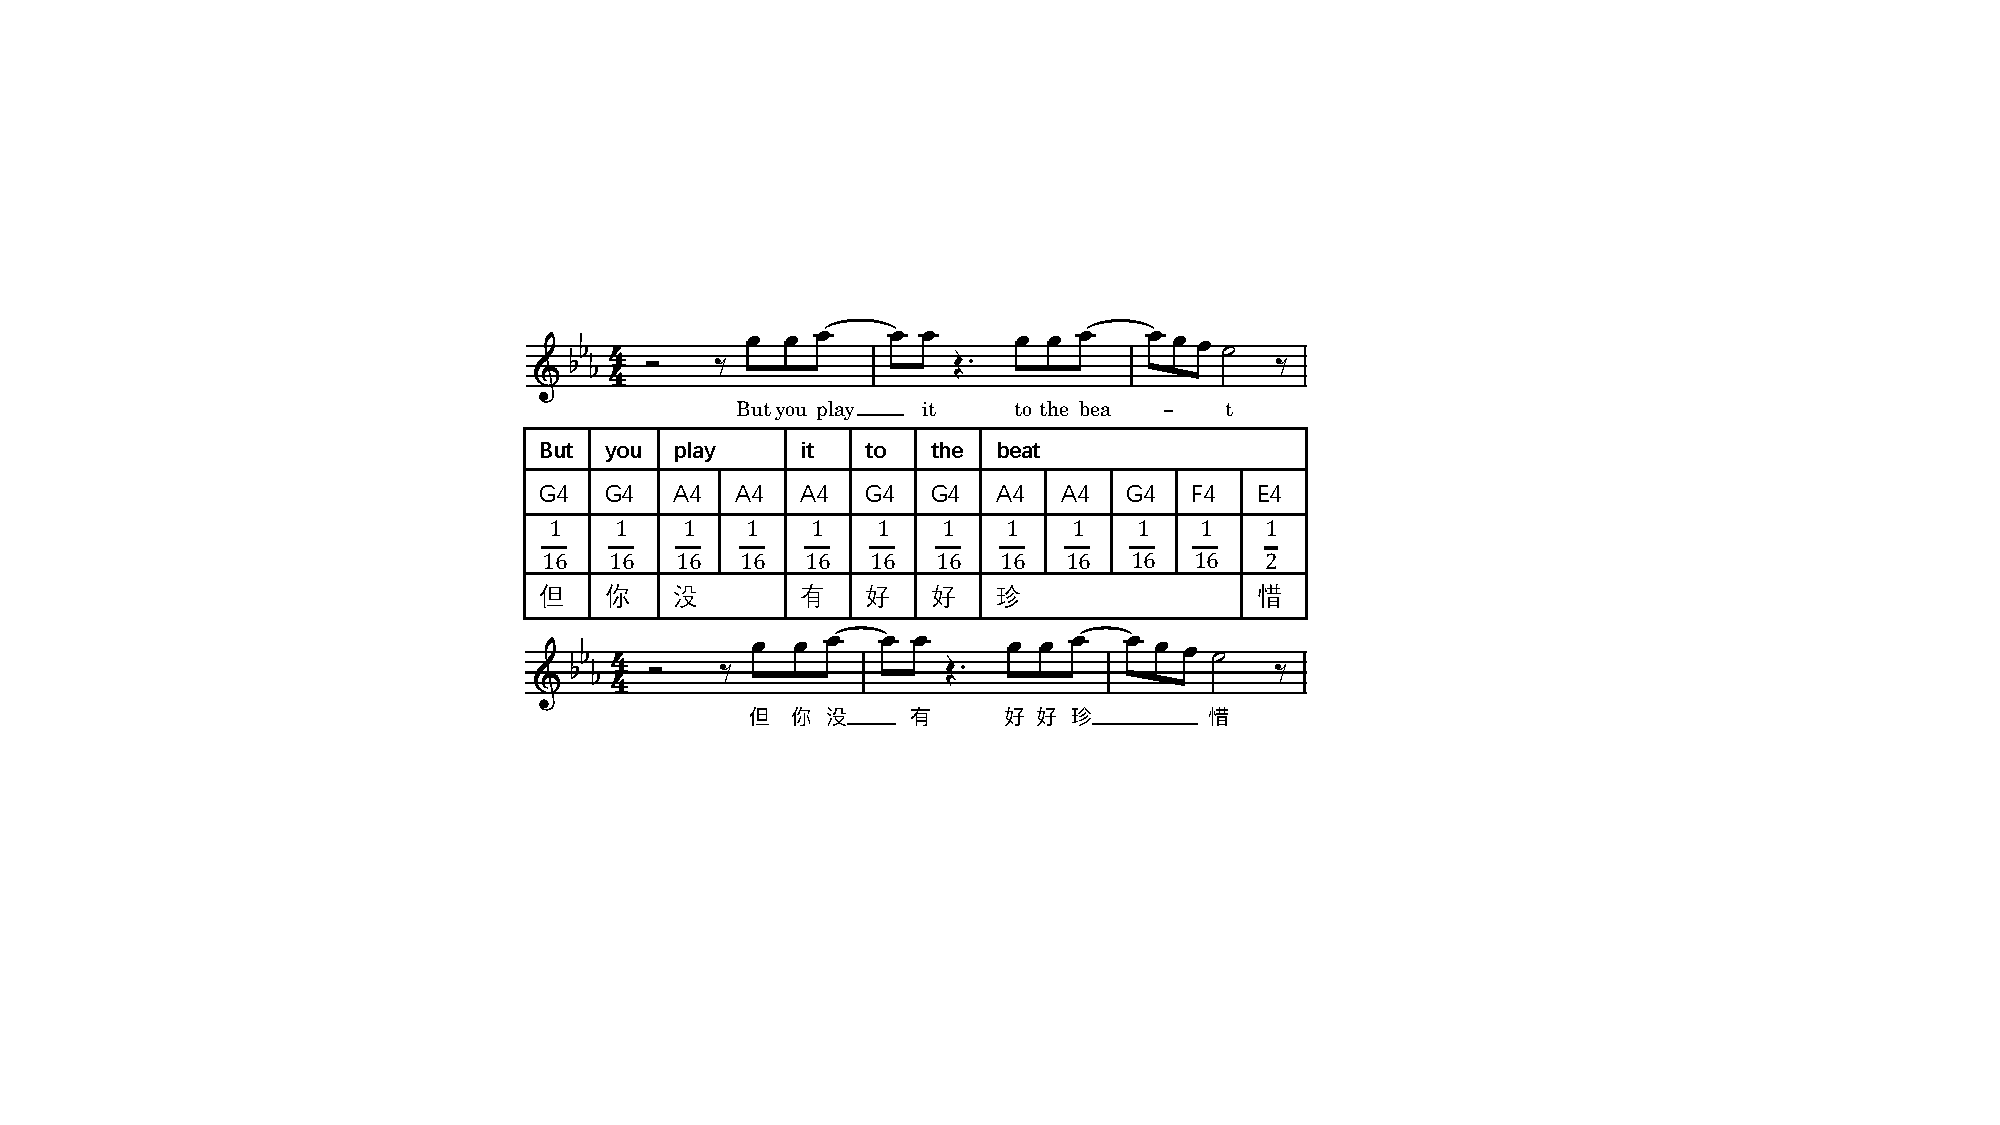
\includegraphics[width=0.99\textwidth]{figure/ast/exp.pdf}
  \caption{以\textit{Rolling In the Deep}一曲中``But you play it to the beat''一句的完整歌曲翻译为例。}
  \label{fig:task_exp}
\end{figure}
然而,尽管机器翻译(Machine Translation,MT)技术,尤其是神经机器翻译~\citep{nmt, vaswani2017attention, hassan2018achieving}(Neural Machine Translation,NMT)的进步,自动歌曲翻译在自然语言处理学界中并未得到充分的研究探索。这其中客观存在的一些挑战包括缺乏收集平行歌词和对齐数据的高效方式、难以对文本和旋律之间的复杂交互进行建模以及没有对乐谱规定的演唱方式进行直观评估的方式。歌曲翻译虽然与文本翻译密切相关,但本质上是一项更复杂的任务。除了在翻译中如用词和词序这样的考虑之外,歌曲的人工翻译者还需要具有目标语言的背景,能理解源语言并作出目标语言中诗意化的表达。此外,如图\ref{fig:task_exp}所示,翻译的歌词需要与旋律合理地对齐来保持歌曲的美感,这是歌曲翻译中不可缺少的要素~\citep{three_d_of_singability}。

此前,学界也探索过歌声合成 (Singing Voice Sythesis,SVS)这一技术来自动化地合成歌曲的人声演唱,并提出了一些在给定歌词和歌谱的情况下产生具有真实人声音色的、自然的、准确的歌声的方法。这样的方法不但使得对歌曲翻译结果方便而直观的评估成为可能,而且也为自动写歌谱曲、自动歌曲翻译这样的研究任务的实际落地奠定了基础。然而,自动歌曲翻译方向上的研究和歌声合成相比很少。作为目前为数不多的工作之一,~\citet{gagast}专注于通过在神经机器翻译的推理过程中施加特定约束来匹配有声调语言的翻译目标词语和旋律的音调、节奏等来得到更加合适、不易造成误解的翻译歌词。然而,\citet{gagast}直接使用文本翻译模型并对音符和字符之间对齐的严格规定一对一的匹配,无法捕捉到歌曲翻译更复杂的本质——即歌词和歌词-旋律对齐之间的关系。虽然音符的数量可以当作是翻译长度的一个简单上限,但正如\citet{interplay_lyrics_melody}一文中所观察到的现象,歌词和旋律之间的微妙对齐不应仅为简单而严格的规则所决定。


为了解决上述技术挑战,我们提出了带有自适应分组的歌词-旋律共同翻译模型,这是自动歌词翻译问题的第一个完整的技术解决方案,通过在基于Transformer的编码器-解码器框架内对歌词翻译和歌词-旋律对齐进行联合建模,我们提出的模型翻译出的歌曲既忠实于原歌词,又符合旋律,无论是客观指标还是主观评测都显示出模型翻译表现的优越性。
\section{章节安排}
本文各章节组织如下:


第一章:绪论。第一章节主要介绍了歌曲翻译技术和歌声合成技术的定义、应用和发展情况、自动歌曲翻译和歌声合成的国内外研究现状、以及自动歌曲翻译和歌声合成的研究背景及意义。另外,第一章节还阐述了本文将基于Transformer Encoder-Decoder模型和歌词和歌词-旋律对齐的关系来研究自动歌曲翻译任务、基于扩散模型来研究歌声合成任务,并探究xxx对于自动歌曲翻译和xxx对于歌声合成效果的影响。

第二章:相关研究介绍。

第三章:自动歌曲翻译研究

第四章:基于扩散模型的歌声合成研究。

第五章:歌曲到歌声翻译系统实践。

第六章:总结和展望。
\section{章节小结}
